\normaltrue
\correctionfalse

%\UPSTIidClasse{12} % 11 sup, 12 spé
%\newcommand{\UPSTIidClasse}{12}

\exer{Mouvement R  $\star$ \label{C2:09:02}}
\setcounter{question}{0}\marginnote{\xpComp{DYN}{06}}%\UPSTIcompetence{C2-09}
\index{Compétence C2-09}\index{Compétence DYN-06}
\index{Principe fondamental de la dynamique}
\index{PFD}
\index{Mécanisme à 1 rotation}
\ifcorrection
\else
\marginnote{\textbf{Pas de corrigé pour cet exercice.}}
\fi

\ifprof
\else
Soit le mécanisme suivant. On a $\vect{AB}=R\vect{i_1}$ avec $R=\SI{20}{mm}$. La liaison pivot est motorisée par un moteur modélisée dont l'action mécanique sur \textbf{1} est donnée par $\vect{C_m}=C_m \vect{k_0}$.
On note $m_1$ la masse du solide \textbf{1} et $B$ son centre d'inertie. 
 La pesanteur est telle que $\vect{g}=-g\vect{j_0}$.
On note $m_1$ la masse du solide 1, $B$ son centre d'inertie et $\inertie{G}{1}=\matinertie{A_1}{A_1}{A_1}{0}{0}{0}{\bas{1}}$.

\begin{marginfigure}
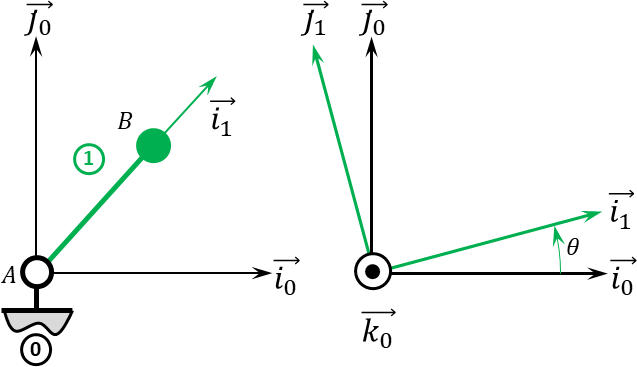
\includegraphics[width=\linewidth]{02_R_01}
\end{marginfigure}

\fi
\question{Dans le but d'obtenir la loi de mouvement, appliquer le théorème du moment dynamique au solide \textbf{1} au point $A$ en projection sur $\vect{k_0}$.}
\ifprof
\else
\fi



\ifprof
\else

\marginnote{Corrigé voir \ref{C2:09:02}.}

\fi